\documentclass[12pt,a4paper,draft]{article}
\usepackage[utf8]{inputenc}
\usepackage[T1]{fontenc}
\usepackage{amsmath}
\usepackage{amsfonts}
\usepackage{amssymb}
\usepackage{graphicx}
\usepackage[width=0.00cm, left=3.00cm, right=2.00cm, top=3.00cm, bottom=2.00cm]{geometry}
\usepackage{venndiagram}
\title{Lista 1}
\date{}
\begin{document}
	\maketitle
	\begin{center}
		\textbf{Curso de Ciências atuariais}\\
		\textbf{Disciplina Probabilidade 1- Professora Cristina}\\
		\textbf{Lista 1- Exercícios de Teoria dos conjuntos (retirado de provas de concurso)}
	\end{center}
	1) A união dos conjuntos A = \{x|x é um número primo e 1 < x < 10\} e B = \{1, 3, 5, 7\} é dada	por:
	\vspace{0.5cm}
	\begin{center}
		A = \{x|x é um número primo e 1 < x < 10\} = \{2, 3, 5, 7\}
		\vspace{0.5cm}\\
		A $\cup$ B = \{1, 2, 3, 5, ,7\}
	\end{center}
	\vspace{1cm}
	2) Represente os conjuntos A = \{- 3, - 1, 0, 1, 6, 7\} , B = \{- 4, 1, 3, 5, 6, 7\} e\\ C = \{- 5, - 3, 1, 2,	3, 5\} no diagrama de Venn e em seguida determine:\\
	\vspace{0.5cm}
	\begin{center}
		\begin{venndiagram3sets}[labelOnlyA={-1 0}, labelOnlyB={-4}, labelOnlyC={-5}, labelOnlyAB={6 7}, labelOnlyAC={-3}, labelOnlyBC={3 5}, labelABC={1}]
		\end{venndiagram3sets}
	\end{center}
	a) A $\cap$ B
	\vspace{0.5cm}
	\begin{center}
		A $\cap$ B = \{1, 6, 7\}
		\vspace{0.5cm}\\
		\begin{venndiagram3sets}[labelOnlyA={-1 0}, labelOnlyB={-4}, labelOnlyC={-5}, labelOnlyAB={6 7}, labelOnlyAC={-3}, labelOnlyBC={3 5}, labelABC={1}]
		\fillACapB
		\end{venndiagram3sets}
	\end{center}
	\vspace{1cm}
	b) C $\cup$ B
	\vspace{0.5cm}
	\begin{center}
		C $\cup$ B = \{-5, -4, -3, 1, 3, 5, 6, 7\}
		\vspace{0.5cm}\\
		\begin{venndiagram3sets}[labelOnlyA={-1 0}, labelOnlyB={-4}, labelOnlyC={-5}, labelOnlyAB={6 7}, labelOnlyAC={-3}, labelOnlyBC={3 5}, labelABC={1}]
			\fillB
			\fillC
		\end{venndiagram3sets}
	\end{center}
	\vspace{1cm}
	c) C – A
	\vspace{0.5cm}
	\begin{center}
		C - A = \{-5, 2, 3, 5\}
		\vspace{0.5cm}\\
		\begin{venndiagram3sets}[labelOnlyA={-1 0}, labelOnlyB={-4}, labelOnlyC={-5}, labelOnlyAB={6 7}, labelOnlyAC={-3}, labelOnlyBC={3 5}, labelABC={1}]
			\fillCNotA
		\end{venndiagram3sets}
	\end{center}
	\vspace{1cm}
	d) B $\cap$ (A $\cup$ C)
	\vspace{0.5cm}
	\begin{center}
		B $\cap$ (A $\cup$ C) = \{1, 3, 5, 6, 7\}
		\vspace{0.5cm}\\
		\begin{venndiagram3sets}[labelOnlyA={-1 0}, labelOnlyB={-4}, labelOnlyC={-5}, labelOnlyAB={6 7}, labelOnlyAC={-3}, labelOnlyBC={3 5}, labelABC={1}]
			\fillCCapB
			\fillACapB
		\end{venndiagram3sets}
	\end{center}
	\vspace{1cm}
	3) Observe a área hachurada da figura e marque a alternativa que a representa.\\
	\vspace{0.5cm}
	\begin{center}
		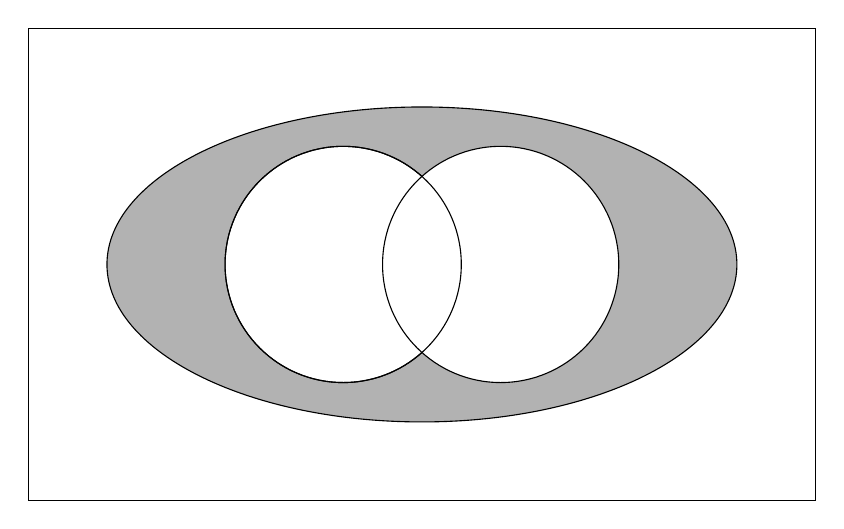
\begin{tikzpicture}
			\draw(-5,-3) rectangle (5cm, 3cm);
			\draw[fill=gray!60](0,0) ellipse (4cm and 2cm);
			\draw[fill=white](-1,0) circle (1.5cm);
			\draw[fill=white](1,0) circle (1.5cm);
			\draw(-1,0) circle (1.5cm);
		\end{tikzpicture}
	\end{center}
	\vspace{0.5cm}
	a) C $\cup$ (A $\cap$ B)\\
	b) C – (A  $\cup$   B)\\
	\textbf{c) C  $\cup$   (A – B)}\\
	d) C $\cap$ (A  $\cup$   B)\\
	\vspace{1cm}\\
	4) De 200 pessoas que foram pesquisadas sobre suas preferências em assistir aos campeonatos de corrida pela televisão, foram colhidos os seguintes dados: 55 dos entrevistados não assistem;	101 assistem às corridas de Fórmula 1; 27 assistem às corridas de Fórmula 1 e de Motovelocidade. Quantas das pessoas entrevistadas assistem, exclusivamente, às corridas de Motovelocidade?
	\vspace{0.5cm}\\
	a) 32\\
	\textbf{b) 44}\\
	c) 56\\
	d) 28\\
	\vspace{0.5cm}
	\begin{center}
	Conjunto Universo $\rightarrow$ U = 200\\
	Não assistem nada $\rightarrow$ N = 55\\
	Assistem aos dois $\rightarrow$ D = 27\\
	Assistem só Fórmula 1 $\rightarrow$ F = 101 - 27 = 74\\
	Assistem só Motovelocidade $\rightarrow$ M = 200 - (55 + 74 + 27) = 200 - 156 = 44
	\end{center}
\end{document}